\section{Methods}

\subsection{Modelization}

In engineering at large (not just robotics), the motivation for modelization is to abstract the (real physical) system of interest into a mathematical object that can be used, calculated upon, and simulated upon.
Examples include modelizing the working of motor by an electrical circuit; modelizing the working of a pump by a fluid circuit; modelizing a plant by a control system, etc$\dots$

\vspace{\baselineskip}

The benefits are two-fold.
The process of modelizing forces the engineer to understand the system, and what parts of the system are relevant to the engineer's work; and upon completion, it also allows the engineer to apply mathematical tools to its system, like control design, simulation, etc$\dots$

\vspace{\baselineskip}

In the field of robotics, modelization's end product are the kinematics and dynamics of the robot.
That modelization doesn't have to be done from scratch, because tools are at disposal, that help both in modelizing the robot, and in unifying its representation (like the urdf format, for example).
However, for this project, the modelization is done from scratch for academic value.

\vspace{\baselineskip}

The starting point is the Figure~\ref*{fig::model}, because in our case, there is no physical robot, only a theoretical generic three-link 2D biped model.

\subsubsection{Kinematics}

% generate kinematics.mlx
% visualize.m

The kinematics of the robot consist in the equations for the positions $\mathbf{x}_i = \begin{pmatrix}
	x_i \\ z_i
\end{pmatrix}$ of the robot links and their respective velocities $\text{d}\mathbf{x}_i$ expressed in relation to the generalized coordinates $\mathbf{q} = \begin{bmatrix}
q_1 \\ q_2 \\ q_3
\end{bmatrix}$ and their derivative $\text{d}\mathbf{q}$:

\begin{align*}
	x_1 &= \dfrac{l_{1}\,\sin\left(q_{1}\right)}{2} \\
	x_2 &= l_{1}\,\sin\left(q_{1}\right)-\dfrac{l_{2}\,\sin\left(q_{2}\right)}{2} \\
	x_3 &= l_{1}\,\sin\left(q_{1}\right)+\dfrac{l_{3}\,\sin\left(q_{3}\right)}{2} \\
	z_1 &= \dfrac{l_{1}\,\cos\left(q_{1}\right)}{2} \\
	z_2 &= l_{1}\,\cos\left(q_{1}\right)-\dfrac{l_{2}\,\cos\left(q_{2}\right)}{2} \\
	z_3 &= l_{1}\,\cos\left(q_{1}\right)+\dfrac{l_{3}\,\cos\left(q_{3}\right)}{2} \\
	\text{d}x_1 &= \dfrac{\mathrm{dq}_{1}\,l_{1}\,\cos\left(q_{1}\right)}{2} \\
	\text{d}x_2 &= \mathrm{dq}_{1}\,l_{1}\,\cos\left(q_{1}\right)-\dfrac{\mathrm{dq}_{2}\,l_{2}\,\cos\left(q_{2}\right)}{2} \\
	\text{d}x_3 &= \mathrm{dq}_{1}\,l_{1}\,\cos\left(q_{1}\right)+\dfrac{\mathrm{dq}_{3}\,l_{3}\,\cos\left(q_{3}\right)}{2} \\
	\text{d}z_1 &= -\dfrac{\mathrm{dq}_{1}\,l_{1}\,\sin\left(q_{1}\right)}{2} \\
	\text{d}z_2 &= \dfrac{\mathrm{dq}_{2}\,l_{2}\,\sin\left(q_{2}\right)}{2}-\mathrm{dq}_{1}\,l_{1}\,\sin\left(q_{1}\right) \\
	\text{d}z_3 &= -\mathrm{dq}_{1}\,l_{1}\,\sin\left(q_{1}\right)-\dfrac{\mathrm{dq}_{3}\,l_{3}\,\sin\left(q_{3}\right)}{2}
\end{align*}

A quick visualization allows to assess visually that the kinematics are correct:

\begin{figure}[H]
	\begin{center}
		\includegraphics[angle=0,width=0.5\textwidth]{a02_visualization}
	\end{center}
	\caption{Visualization of the kinematics of the three-link 2D biped model.}
\end{figure}

\subsubsection{Dynamics}

% generate dynamics.mlx
% eval M.m, eval C.m, eval G.m, eval B.m

Computing the dynamics means computing the mass matrix $\mathbf{M}$, Coriolis matrix $\mathbf{C}$, gravity vector $\mathbf{G}$ and control matrix $\mathbf{B}$ for the robot, from the kinematics, using the Lagrangian method.
This allows to have the equation of motion for the robot:

\begin{align}
	\label{eq::motion_eq}
	\mathbf{M}\left(\mathbf{q}\right)\mathbf{\ddot{q}} + \mathbf{C}\left(\mathbf{q},\mathbf{\dot{q}}\right)\mathbf{\dot{q}} + \mathbf{G}\left(\mathbf{q}\right) &= \mathbf{Bu}
\end{align}

The first step is to compute the Langrangian of the system:

\begin{align*}
	\underbrace{L}_\text{Lagrangian} &= \underbrace{T}_\text{total kinetic energy} - \underbrace{V}_\text{total potential energy} \\
	&= \left(T_1+T_2+T_3\right) - \left(V_1+V_2+V_3\right) \\
	&= \sum_{i=1}^{3} \dfrac{1}{2} m_i \mathbf{\dot{x}}^2 - \sum_{i=1}^{3} m_i g z_i \\
\end{align*}

with $i$ denoting the links of the robot.

\vspace{\baselineskip}

The Lagrange equation states that:

\begin{equation*}
	\dfrac{\text{d}}{\text{d}t}\left(\dfrac{\partial L}{\partial \dot{q}_i}\right) = \dfrac{\partial L}{\partial q_i}
\end{equation*}

From this last equation, the matrices $\mathbf{M}$, $\mathbf{C}$ and $\mathbf{G}$ are deduced by substitution.
To verify that the substitution is correct, the error on the following is computed (and the error should amount to zero, obviously):

\begin{equation*}
	\left( \mathbf{M}\left(\mathbf{q}\right)\mathbf{\ddot{q}} + \mathbf{C}\left(\mathbf{q},\mathbf{\dot{q}}\right)\mathbf{\dot{q}} + \mathbf{G}\left(\mathbf{q}\right) \right) - \left( \dfrac{\text{d}}{\text{d}t}\left(\dfrac{\partial L}{\partial \dot{q}_i}\right) - \dfrac{\partial L}{\partial q_i}
	\right)
\end{equation*}

Then, the control matrix $\mathbf{B}$ is computed. The robot is commanded through $\mathbf{u}_1$ and $\mathbf{u}_2$ as described on Figure~\ref*{fig::model_with_command} below:

\begin{figure}[H]
	\begin{center}
		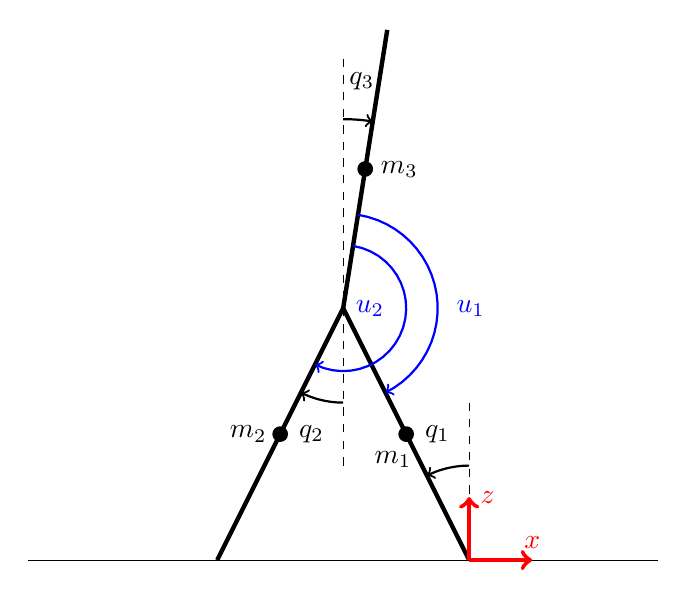
\begin{tikzpicture}
			\begin{scope}[x={8cm},y={8cm}]
				% l = 0,447213
				% alpha = 8.999999999478607 deg
				% =0.5+sqrt(0.2^2+0.4^2)*sin(pi/20)
				% =0.4+sqrt(0.2^2+0.4^2)*cos(pi/20)

				\draw[-] (0,0)--(1,0); % ground

				\draw[-,ultra thick] (0.3,0)--(0.5,0.4); % link 2
				\draw[-,ultra thick] (0.7,0)--(0.5,0.4); % link 1
				\draw[-,ultra thick] (0.5,0.4)--(0.5699596195707541,0.8417076540309386); % link 3

				\draw[dashed] (0.5,0.15)--(0.5,0.8); % big vertical dashed line
				\draw[dashed] (0.7,0)--(0.7,0.25); % small vertical dashed line

				\draw[->,ultra thick, red] (0.7,0)--(0.8,0) node[above]{$x$}; % x axis
				\draw[->,ultra thick, red] (0.7,0)--(0.7,0.1) node[right]{$z$}; % y axis

				\draw [->,thick,domain=81.00000000052139:-63.4349488, blue] plot ({0.5+0.15*cos(\x)}, {0.4+0.15*sin(\x)}); % u1
				\draw [->,thick,domain=81.00000000052139:-116.5650512, blue] plot ({0.5+0.10*cos(\x)}, {0.4+0.10*sin(\x)}); % u2

				\draw [->,thick,domain=-90:-116.5650512] plot ({0.5+0.15*cos(\x)}, {0.4+0.15*sin(\x)}); % q2
				\draw [->,thick,domain=90:116.5650512] plot ({0.7+0.15*cos(\x)}, {0.15*sin(\x)}); % q1
				\draw [->,thick,domain=90:81.00000000052139] plot ({0.5+0.3*cos(\x)}, {0.4+0.3*sin(\x)}); % q3

				\node at (0.4,0.2) [circle,fill,inner sep=1]{.}; % m2
				\node at (0.6,0.2) [circle,fill,inner sep=1]{.}; % m1
				\node at (0.5349798097853771,0.6208538270154693) [circle,fill,inner sep=1]{.}; % m3

				\node[text width=0mm] at (0.63,0.2) {$q_1$};
				\node[text width=0mm] at (0.43,0.2) {$q_2$};
				\node[text width=0mm] at (0.51,0.76) {$q_3$};

				\node[text width=0mm] at (0.55,0.16) {$m_1$};
				\node[text width=0mm] at (0.32,0.2) {$m_2$};
				\node[text width=0mm] at (0.56,0.62) {$m_3$};

				\node[text width=0mm, blue] at (0.68,0.4) {$u_1$};
				\node[text width=0mm, blue] at (0.52,0.4) {$u_2$};
			\end{scope}
		\end{tikzpicture}
	\end{center}
	\caption{Representation of the three-link 2D biped model with its generalized coordinates $\mathbf{q}$ and command angles $\mathbf{u}$.}
	\label{fig::model_with_command}
\end{figure}

This means that the model is underactuated, because there is more DOFs ($q_1$, $q_2$, $q_3$) than actuated joints ($u_1$, $u_2$).

\vspace{\baselineskip}

The work done by $\mathbf{u}_1$ and $\mathbf{u}_2$ is computed as the product of $\mathbf{u}_i$ and the corresponding virtual angle variation.
Then, the control matrix is computed by substitution.

\vspace{\baselineskip}

The obtained matrices are:

\begin{align*}
	\mathbf{M} &= \begin{bmatrix}
		{l_{1}}^2\,\left(\dfrac{m_{1}}{4}+m_{2}+m_{3}\right) & -\dfrac{l_{1}\,l_{2}\,m_{2}\,\cos\left(q_{1}-q_{2}\right)}{2} & \dfrac{l_{1}\,l_{3}\,m_{3}\,\cos\left(q_{1}-q_{3}\right)}{2}\\ -\dfrac{l_{1}\,l_{2}\,m_{2}\,\cos\left(q_{1}-q_{2}\right)}{2} & \dfrac{{l_{2}}^2\,m_{2}}{4} & 0\\ \dfrac{l_{1}\,l_{3}\,m_{3}\,\cos\left(q_{1}-q_{3}\right)}{2} & 0 & \dfrac{{l_{3}}^2\,m_{3}}{4}
	\end{bmatrix} \\
	\mathbf{C} &= \begin{bmatrix}
		0 & -\dfrac{\mathrm{dq}_{2}\,l_{1}\,l_{2}\,m_{2}\,\sin\left(q_{1}-q_{2}\right)}{2} & \dfrac{\mathrm{dq}_{3}\,l_{1}\,l_{3}\,m_{3}\,\sin\left(q_{1}-q_{3}\right)}{2}\\ \dfrac{\mathrm{dq}_{1}\,l_{1}\,l_{2}\,m_{2}\,\sin\left(q_{1}-q_{2}\right)}{2} & 0 & 0\\ -\dfrac{\mathrm{dq}_{1}\,l_{1}\,l_{3}\,m_{3}\,\sin\left(q_{1}-q_{3}\right)}{2} & 0 & 0
	\end{bmatrix} \\
	\mathbf{G} &= \begin{bmatrix}
		-\dfrac{g\,l_{1}\,\sin\left(q_{1}\right)\,\left(m_{1}+2\,m_{2}+2\,m_{3}\right)}{2}\\ \dfrac{g\,l_{2}\,m_{2}\,\sin\left(q_{2}\right)}{2}\\ -\dfrac{g\,l_{3}\,m_{3}\,\sin\left(q_{3}\right)}{2}
	\end{bmatrix} \\
	\mathbf{B} &= \begin{bmatrix}
		1 & 0\\ 0 & 1\\ -1 & -1
	\end{bmatrix}
\end{align*}

It is interesting to notice that the mass matrix $\mathbf{M}$ corresponds to the Jacobian of the total kinetic energy $T$ with respect to the generalized coordinates.
This result is to be expected, since kinetic energy is derived from moving masses.% (\textbf{assignment 1 question}).

\subsubsection{Impact map}

% generate impact map.mlx (in the “generate model” folder)
% eval A m.m, eval A p.m (in the “dynamics” folder)
% impact.m (in the “dynamics” folder)

In the hybrid model of walking, the model oscillates between the single support swing phase and the impact phase, during which the leg roles are switched, like so:

\begin{center}
	\begin{tikzpicture}[auto]
		\node [block] (swing) {Single support swing phase};
		\node [block, right=of swing] (impact) {Impact phase};

		\draw [->] (swing) |- (0, 1.5) -| (impact);
		\draw [<-] (swing) |- (0, -1.5) -| (impact);
	\end{tikzpicture}
\end{center}

The modelization of the swing phase has been extensively described in the previous sections, leading to the kinematics and dynamics of the robot during the single support swing phase through the Lagrangian method.

\vspace{\baselineskip}

This section is concerned with the impact phase.
This phase is based on the assumptions that:

\begin{itemize}
	\item the impact and leg role switching is instantaneous and
	\item the support leg does not slip.
\end{itemize}

Because of the assumption of instantaneousness, there is no need for (and it would prove to be quite difficult to) develop kinematics and dynamics for the impact phase.
Instead, the state of the robot is mapped from right before the impact to right after the impact, throught the use of the impact map $\mathbf{\Delta}$ computed by conservation of the angular momentum.
In particular, we can write:

\begin{align*}
	\mathbf{\Delta} \left( \mathbf{q}_m, \mathbf{\dot{q}}_m \right) &= \begin{bmatrix}
		\mathbf{\Delta}_q \left( \mathbf{q}_m \right) &  \mathbf{\Delta}_{\dot{q}} \left( \mathbf{q}_m, \mathbf{\dot{q}}_m \right)
	\end{bmatrix}
\end{align*}

The angular positions are the same (semantically) before and after impact, so their mapping $\mathbf{\Delta}_q \left( \mathbf{q}_m \right)$ only needs to account for the change of reference frame.

\vspace{\baselineskip}

On the contrary, the angular velocities after impact are computed using the McGeer method~\cite{mcgeer}, which is a conservation of angular momentum method: the angular momentum before impact $H_m$ must be equal to the angular momentum after impact $H_p$:

\begin{align*}
	H_m &= H_p \\
	A_m\mathbf{\dot{q}}_m &= A_p\mathbf{\dot{q}}_p \\
	\mathbf{\dot{q}}_p &= A_{p}^{-1}A_m\mathbf{\dot{q}}_m
\end{align*}

After computation:

\tiny

\begin{align*}
	A_p &= \begin{bmatrix}
		\dfrac{l_{1}\,l_{2}\,m\,\cos\left(q_{1,p}-q_{2,p}\right)}{2}-{l_{1}}^2\,m_{3}-\dfrac{5\,{l_{1}}^2\,m}{4}-\dfrac{l_{1}\,l_{3}\,m_{3}\,\cos\left(q_{1,p}-q_{3,p}\right)}{2} & \dfrac{l_{1}\,l_{2}\,m\,\cos\left(q_{1,p}-q_{2,p}\right)}{2}-\dfrac{{l_{2}}^2\,m}{4} & -\dfrac{m_{3}\,{l_{3}}^2}{4}-\dfrac{l_{1}\,m_{3}\,\cos\left(q_{1,p}-q_{3,p}\right)\,l_{3}}{2}\\ \dfrac{l_{1}\,l_{2}\,m_{3}\,\cos\left(q_{1,p}-q_{2,p}\right)}{2} & -\dfrac{{l_{2}}^2\,m_{3}}{4} & 0\\ -\dfrac{l_{1}\,l_{3}\,m\,\cos\left(q_{1,p}-q_{3,p}\right)}{2} & 0 & -\dfrac{{l_{3}}^2\,m}{4}
	\end{bmatrix} \\
	A_m &= \begin{bmatrix}
		\dfrac{{l_{1}}^2\,m}{4}-l_{1}\,l_{2}\,m\,\cos\left(q_{1,m}-q_{2,m}\right)-l_{1}\,l_{2}\,m_{3}\,\cos\left(q_{1,m}-q_{2,m}\right)-\dfrac{l_{1}\,l_{3}\,m_{3}\,\cos\left(q_{1,m}-q_{3,m}\right)}{2} & \dfrac{{l_{2}}^2\,m}{4} & -\dfrac{m_{3}\,{l_{3}}^2}{4}-\dfrac{l_{2}\,m_{3}\,\cos\left(q_{2,m}-q_{3,m}\right)\,l_{3}}{2}\\ \dfrac{{l_{1}}^2\,m_{3}}{4} & 0 & 0\\ -\dfrac{l_{1}\,l_{3}\,m\,\cos\left(q_{1,m}-q_{3,m}\right)}{2} & 0 & -\dfrac{{l_{3}}^2\,m}{4}
	\end{bmatrix}
\end{align*}

\normalsize

with $m=m_1=m_2$, and thus both $\mathbf{q}_p$ and $\mathbf{\dot{q}}_p$ can be computed.

\paragraph{Assignment 2 questions}

\begin{enumerate}
	\item \textit{What can you say about the potential energy before and after impact?}

	The potential energy before and after the impact are the same, since the frame of reference is moved from one foot to another without any change in the position, velocity or acceleration of the different masses.

	\item \textit{Try $\mathbf{q}_m = \begin{bmatrix}
		pi/6 & -pi/6 & pi/10
	\end{bmatrix}$, $\mathbf{\dot{q}}_m = \begin{bmatrix}
		1 & 0.2 & 0
	\end{bmatrix}$. What percentage of the kinetic energy of the biped is lost due to the impact?}

	Computing using our functions, we find that 38.73\% of the kinetic energy is lost during the impact of the foot for those parameters.

	\item \textit{Plot the percentage of the kinetic energy loss due to impact as a function of angle $\alpha$ where $\mathbf{q}_m=\begin{bmatrix}
		\alpha & -\alpha & 0
	\end{bmatrix}$ and $\alpha$ varies from 0 to $\pi/4$. Assume that $\mathbf{\dot{q}} = \begin{bmatrix}
		1 & 0.2 & 0
	\end{bmatrix}$.}

	\begin{figure}[H]
		\begin{center}
			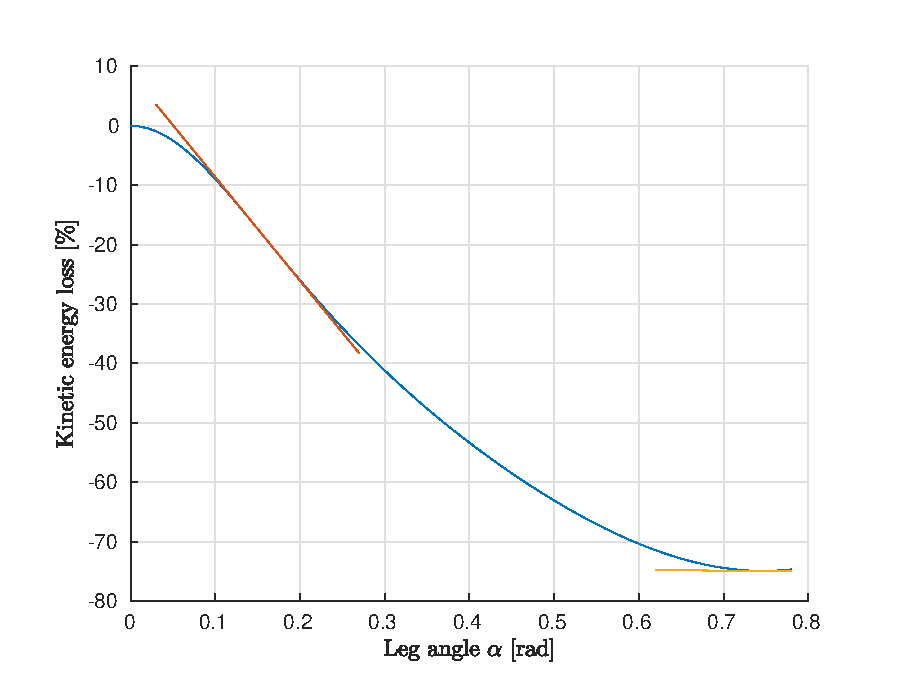
\includegraphics[angle=0,width=0.7\textwidth]{a02_kinetic_energy_loss_along_leg_angle}
		\end{center}
		\caption{Percentage of kinetic energy loss as a function of leg angle.}
	\end{figure}

	\item \textit{The bigger $\alpha$ is, the bigger is the step length. Based on your answer to question 3, what is the relation between step length and energy loss at impact given a fixed $\mathbf{\dot{q}}_m$?}

	The bigger the step, the bigger the energy loss: if there is no step at all (i.e. if $\alpha=0$), there is no energy loss.
	From $\alpha=0$ to $\alpha=\SI{0.15}{\radian}$, the loss rate in kinetic energy increases.
	From $\alpha=\SI{0.15}{\radian}$ to $\alpha=\SI{0.74}{\radian}$, the loss rate in kinetic energy decreases.
\end{enumerate}

\subsection{Simulation}

In the introduction, the control design pipeline was described in three steps.
After the modelling step that has been discussed in the previous section, there is the simulation step.
The idea is to translate the (second order) equations of motion, Equation~\ref{eq::motion_eq} that describes the swing phase, into first order differential equations, in order to solve them numerically.
The discrete events of impact with the ground can be dealt with an event function that interrupts the integrator of the numerical integration when impact conditions are met.
When impact is dealt with, the integrator is given new "initial conditions" and numerical integration is resumed.

\subsubsection{Equations of motion}
% eqns.m
% event func.m
% solve eqns.m

To translate the second order equation of motion into a first order differential equation, first, let's define $\mathbf{y}$ as follows:

\begin{align}
	\label{eq::angle_solution}
	\mathbf{y} &= \begin{bmatrix}
		\mathbf{y}_1 \\ \mathbf{y}_2
	\end{bmatrix} = \begin{bmatrix}
		\mathbf{q} \\ \mathbf{\dot{q}}
	\end{bmatrix}
\end{align}

From which, with Equation~\ref{eq::motion_eq}, it follows that:

\begin{align*}
	\mathbf{\dot{y}} &= \begin{bmatrix}
		\mathbf{\dot{q}} \\ \mathbf{\ddot{q}}
	\end{bmatrix} \\
	&= \begin{bmatrix}
		\mathbf{y}_2 \\ \mathbf{M}^{-1} \left( \mathbf{y}_1 \right) \left( \mathbf{Bu} - \mathbf{C} \left( \mathbf{y}_1, \mathbf{y}_2 \right) \mathbf{y}_2 + \mathbf{G} \left( \mathbf{y}_1 \right) \right)
	\end{bmatrix}
\end{align*}

The event function taking care of the impact with the ground triggers when the swing foot hits
the ground with a negative vertical velocity.

\vspace{\baselineskip}

The numerical solution is computed by \verb|ode45|.

\subsubsection{Animation}
% animate.m (in the “visualize” folder)

Then, the idea is to extract join coordinates $\mathbf{q}$ from the solution computed by \verb|ode45| as described by Equation~\ref{eq::angle_solution} (the numerical integration provides a solution vector for $\mathbf{y}$), in order to obtain a graphical animation of the three-link 2D biped model.

\paragraph{Assignment 3 questions}

\begin{enumerate}
	\item \textit{In the animations, what does a real-time factor of 1 mean? How about a real-time factor less than 1?}

	The real time factor is the actual duration of the simulations (obtained from \verb|sln|) divided by the time it takes for MATLAB to animate the simulations (obtained from \verb|t_anim|).
	With a real-time factor of 1 or greater, the animation is done in "real-time".
	With a real-time factor lesser than 1, the computation is more slow than "real-time".
	\verb|real_time_factor| is a non-null positive value, but having one greater than 1 has no use, because even when the computation happens faster, the displaying doesn't.

	\item \textit{How does "skip" in animate.m effect the real-time factor and the speed of the animation?}

	Skip allow to skip a few step, so the animation can go faster.
	It affects the real time factor because less steps are computed for the same time vector, so that it improves the real time factor.

	\item \textit{What is the role of} \verb|r0| \textit{in animate.m?}

	It is the foot position, so it has to be updated at each cycle, by accumulating \verb|x_swf|, which is the swing foot position increase.
\end{enumerate}

\subsubsection{Numerical integration}
% numerical integration.zip

Numerical integration is handy tool for engineers to calculate a number of numerical values, and amongst others, numerical solutions to differential equations. However handy, numerical integration as a field as its subtleties, and solutions should be carefully examined before being applied to problems (especially stiff problems).
Let's discuss some of the more common numerical integration algorithms.

\paragraph{Explicit Euler}

\begin{enumerate}
	\item \textit{Explain the meaning of the state-space plot. What should be the expected state-space plot?}

	The state-space plot displays the position against the speed.
	Because the analytical solution for the position is sinusoidal, the speed is also sinusoidal, albeit with a phase shift of \SI{\pi/2}{\radian}, so that the state-space should display a circle.
	The fact that it displays an outward spirals shows that the solution diverges.
	Generally speaking, a state-space plot that is closed (or ends up closed) describes a stable system or solution, while a state-space plot that is not closed, describes a diverging system or solution.

	\item \textit{Why does the numerical solution diverges from the true solution?}

	The explicit Euler numerical integration is a first order approximation of the Taylor series.
	Here, the position is a cosine, and so the speed is a sine.
	The absolute value of the first order Taylor approximation of a sine ($\sin x \sim x$) is always bigger than the approximated value (that is, $|x|>|\sin x|$), so that the state-space plot cannot be a circle, and in fact diverges into a spiral.

	\item \textit{What can you do to better approximate the actual solution with this method?}

	When the step size $dt$ is reduced, the error between an analytical solution and the numerical approximation diminishes:

	\begin{figure}[H]
		\begin{subfigure}[h]{\textwidth}
			\begin{center}
				\includegraphics[angle=0,width=0.7\textwidth]{num_int_exp_euler_01}
				\caption{$dt=0.1$}
			\end{center}
		\end{subfigure}

		\begin{subfigure}[h]{\textwidth}
			\begin{center}
				\includegraphics[angle=0,width=0.7\textwidth]{num_int_exp_euler_001}
				\caption{$dt=0.01$}
			\end{center}
		\end{subfigure}
		\caption{Numerical and analytical solutions and state-space plot to $m y'' + d y' + k y =0$ with the explicit Euler method.}
	\end{figure}

	That's because the local truncation error for the explicit Euler method is $\text{LTE} = \dfrac{1}{2}dt^2y''(t_0)+O(dt^3)$, so that when $dt$ decreases, so does the LTE (and thus the GTE, the global truncation error).
\end{enumerate}

\paragraph{Semi-implicit Euler}

\begin{enumerate}
	\item \textit{Is this method stable and when?}

	This method is stable for complex roots of the characteristic equation within the circle defined by $s>-\dfrac{2}{dt}$.
	For real roots, the solution is always stable.
	In this particular instance, the state-space plot is closed, so the solution is stable.

	\item \textit{What about the accuracy of the obtained solution?}

	The semi-implicit Euler numerical method is a first-order integrator, just like the explicit Euler method, but the use of $u(t_0+dt)$ instead of $u(t_0)$ in the equation for $y(t_0+dt)$ makes it more accurate than the explicit Euler method, as can be assessed visually when comparing (for fixed parameters):

	\begin{figure}[H]
		\begin{subfigure}[h]{\textwidth}
			\begin{center}
				\includegraphics[angle=0,width=0.7\textwidth]{num_int_exp_euler_001}
				\caption{explicit Euler method}
			\end{center}
		\end{subfigure}

		\begin{subfigure}[h]{\textwidth}
			\begin{center}
				\includegraphics[angle=0,width=0.7\textwidth]{num_int_semi_imp_euler_001}
				\caption{semi-implicit Euler method}
			\end{center}
		\end{subfigure}
		\caption{Numerical and analytical solutions and state-space plot to $m y'' + d y' + k y =0$ with $dt=0.01$.}
	\end{figure}
\end{enumerate}

\paragraph{Runge-Kutta of Order 4 (Midpoint Method)}

\begin{enumerate}
	\item \textit{What is the error of this method?}

	The LTE of RK4 is $O(dt^4)$, and thus the GTE is $O(dt^3)$.

	\item \textit{Do you expect the solution to diverge?}

	The state-space plot is closed, so the solution doesn't diverge:
	\begin{figure}[H]
		\begin{center}
			\includegraphics[angle=0,width=0.7\textwidth]{num_int_rk4_01}
			\caption{Numerical and analytical solutions and state-space plot to $m y'' + d y' + k y =0$ with $dt=0.1$ and the Runge-Kutta order 4 method.}
		\end{center}
	\end{figure}
\end{enumerate}

\paragraph{Adaptive Time Stepping}

\begin{enumerate}
	\item \textit{Change the density of the time points in np.linspace. What do you observe?}

	When the density of points increases, the solution gains in temporal resolution.

	\begin{figure}[H]
		\begin{subfigure}[h]{\textwidth}
			\begin{center}
				\includegraphics[angle=0,width=0.7\textwidth]{num_int_odeint_02}
				\caption{$dt=0.2$}
			\end{center}
		\end{subfigure}

		\begin{subfigure}[h]{\textwidth}
			\begin{center}
				\includegraphics[angle=0,width=0.7\textwidth]{num_int_odeint_005}
				\caption{$dt=0.05$}
			\end{center}
		\end{subfigure}
		\cprotect\caption{Numerical and analytical solutions and state-space plot to $m y'' + d y' + k y =0$ with \verb|odeint| from \verb|SciPy|.}
	\end{figure}

	\item \textit{Do you expect the solution to diverge?}

	The state-space plot is circular, so the solution doesn't diverge.

	\item \textit{Which algorithms are supported by} \verb|odeint|\textit{?}

	\verb|odeint| uses the LSODA algorithm~\cite{hindmarsh}, which switches automatically between the BDF (stiff) method and the Adams (non-stiff) method, so that the integration is suited to the problem.
\end{enumerate}

\subsection{Control and optimization}

This design of controllers and their optimizations is the third step of control design pipeline. The implementation of three controllers were attempted, with various degrees of success.
The first is the virtual constraints controller, the second, a controller based on reinforcement learning, and the third, a virtual model controller using task space projection.

\subsubsection{Virtual constraints controller}

The first controller designed is a virtual constraints controller.
As indicated by the name, it makes use of constraints that are virtual, and defined mathematically.
Here, two constraints are defined, $y_1$ and $y_2$.
They are a function of the model's coordinates, and represent conditions that helps producing a stable gait.
Thus, the goal is to cancel them by closing the loop with a PD controller.
On Figure~\ref{fig::model_with_command}, it can be seen that the model is under-actuated.
$u_1$ can control both the torso ($q_3$ and $q_1$) and stance foot, while $u_2$ can control both the torso and swing foot ($q_3$ and $q_2$).
Thus a choice has to be made about which generalized coordinates are controlled directly, and which is free to follow the dynamics of the model.
Here it is chosen that $u_1$ directly controls the torso, and indirectly the stance foot, while $u_2$ directly controls the swing foot:

\begin{align*}
	y_1 &= q_3 - \alpha \\
	y_2 &= -q_2-q_1
\end{align*}

where $\alpha$ is the desired lean angle.

The first constraint helps constraining the lean angle to the \textit{desired} lean angle ($q_3\sim\alpha$).

The second constraint helps in keeping the swing and stance leg as balanced / vertically symmetrical as possible ($q_1=-q_2$).

When differentiating with respect to time, it gives:

\begin{align*}
	\dot{y}_1 &= \dot{q}_3 \\
	\dot{y}_2 &= -\dot{q}_2-\dot{q}_1
\end{align*}

And thus a PD controller is expressed like so:

\begin{align*}
	u_1 &= k_{P1}y_1 + k_{D1} \dot{y}_1 \\
	u_2 &= k_{P2}y_2 + k_{D2} \dot{y}_2
\end{align*}

The optimization problem is defined as the objective function $f$ of the decision variables $p$ chosen amongst the model parameters:

\begin{align}
	\label{eq::virtual_constraints_objective_fun}
	f(p) &= w_1 | \dot{x}_\text{hip d} - \bar{\dot{x}}_\text{hip}(p) | + w_2 \text{CMT}(p)
\end{align}

where $\dot{x}_\text{hip d}$ is the desired horizontal hip velocity, $\bar{\dot{x}}_\text{hip} (p)$ the simulated average horizontal velocity, and $w_i$ weights.

\vspace{\baselineskip}

The CMT, Cost of Mechanical Transport is defined through the normalized effort $U$ like so:

\begin{align*}
	\text{CMT} &= \dfrac{U}{x_\text{h}(T)-x_\text{h}(1)} \\
	U &= \dfrac{1}{2TU_\text{max}} \sum_{i=1}^{T} \left( u_{1}^{2} (i) + u_{2}^{2} (i) \right) \\
	U_\text{max} &= \SI{30}{\newton\meter}
\end{align*}

The optimizer goal is to minimize the objective function over the decision variables:

\begin{align*}
	&\underset{p}{\min} f(p)
\end{align*}

while managing the competing aspects of the terms (minimizing the CMT implies decreasing the simulated velocity), as well as achieving appropriate gaits (mathematical optimization doesn't always lead to solutions that make sense in a concrete, physical setup).

\vspace{\baselineskip}

Here, the optimizer's decision variables are:

\begin{itemize}
	\item $\mathbf{q}_0$ and $\mathbf{\dot{q}}_0$,
	\item $k_{p1}$, $k_{p2}$,
	\item $k_{d1}$, $k_{d2}$,
	\item and the leaning angle $\alpha$.
\end{itemize}

\subsubsection{Reinforcement learning controller}

The second attempt was at a reinforcement learning controller.

Reinforcement Learning (RL) is one of the three basic machine learning paradigms alongside supervised and unsupervised learning.
RL can be used to  virtually train a controller to achieve a certain goal.

\vspace{\baselineskip}

By defining an environment in which a robot can pursue a certain set of motions limited by the physics, and guided by a reward function chosen to induce certain behaviours for the robot, an agent tries to optimize a set of inputs in order to maximize the reward, as described on Figure~\ref{fig::rl_workflow}.

\begin{figure}[H]
	\centering
	\includegraphics[angle=0,width=0.6\textwidth]{a05_rl_workflow}
	\caption{Workflow of the Reinforcement Learning algorithm.}
	\label{fig::rl_workflow}
\end{figure}

This method has the advantage of not having to perfectly know the relationship between an input and the system associated behaviour. Only the physics of the environment have to be well defined, as well as the reward function.
It can be expressed as:

\begin{equation*}
	\begin{split}
		\max &\sum^T_{t=0} R_t(x_t,u_t) \\
		\text{s.t. } &x_{t+1} = f(x_t,u_t,e_t)
	\end{split}
\end{equation*}

with $R$ the reward function, and $x_t$, $u_t$ and $e_t$ respectively the state, input and error at instant $t$.
Thus, at each point in time, the agent knows the current and past states of the system, and optimizes a trajectory by choosing the best sequence of future inputs, while mitigating the error through feedback.
How to choose the best course of action is called a policy $\pi$. This policy is what the RL agent optimizes.


For the bipedal robot simulation, the algorithm was supposed to be implemented using MATLAB's toolbox for Reinforcement Learning.
This led to two possibilities, using a MATLAB environment to code the algorithm or Simulink.
Both were tested but Simulink was chosen in the end as it would have allowed us, with a working environment, to switch to another type of controller more easily if Reinforcement Learning was proven to take too long or be too difficult.
The environment made use of the different functions defined during the precedent assignments.
Figure~\ref{fig::rl_main_loop} and Figure~\ref{fig::rl_system_dynamics} displays the content of the Simulink algorithm.

\begin{figure}[H]
	\centering
	\includegraphics[angle=0,width=\textwidth]{a05_rl_main_loop}
	\caption{Main loop of the environment}
	\label{fig::rl_main_loop}
\end{figure}

\begin{figure}[H]
	\centering
	\includegraphics[angle=0,width=\textwidth]{a05_rl_system_dynamics}
	\caption{Dynamic of the system}
	\label{fig::rl_system_dynamics}
\end{figure}

The main issue encountered with this method is the presence of what is called algebraic loops.
Those loops happen when the output of a function necessitates its own future output as an input.
While this should have been easily solved by defining initial conditions, Simulink was struggling with those loops.
Another solution explored was to use a time delay or a memory block, which can solve those loops in most of cases.
However, it delays the dynamic of the system, thus affecting the behavior of the walking robot.
The only possible solution found was to move on from Simulink to Simscape which handles those loops better for dynamical systems.
However this would have taken us even longer and instead, we chose to switch to another type of controller.

\vspace{\baselineskip}

Had it not be that difficult to use Simulink for RL, an actor-critic agent would had been chosen to determine the policy of the controller.
The observation signal would have been the different coordinates of the robot, and the reward function was first thought to be something similar as in~\cite{matlab_rl}:

\begin{equation*}
	R = \dot{x}_\text{hip} - 50 \left( 0.3-z_\text{hip} - \text{CMT} \right)
\end{equation*}

This function rewards the velocity of the robot and penalizes the changes in height and the cost of transport.
This reward function was kept later on for the optimization of the third controller, the virtual model controller.

\subsubsection{Virtual model controller}

Finally, the third controller is a virtual model controller using task space projection.
Virtual model control is a motion control framework that uses virtual components to create virtual forces generated when the virtual components interact with the robot.

\vspace{\baselineskip}

Specifically, the idea is to use both the control matrix $\mathbf{B}$ (obtained from the dynamics of the robot), as well as the Jacobian $\mathbf{J}$ of the robot at specific joints or points of interest of the robot, to compute a control matrix $\mathbf{u}$ that applies chosen virtual forces $\mathbf{f}$ like so:

\begin{align*}
	\mathbf{u} &= \mathbf{B}^+ \mathbf{J}^T \left( \mathbf{q} \right) \mathbf{f} \\
	\text{s.t. } \mathbf{f} &= \begin{bmatrix}
		k_\text{px} \left( x_t - x \right) + k_\text{dx} \left( \dot{x}_t - \dot{x} \right) \\
		k_\text{pz} \left( z_t - z \right) + k_\text{dz} \left( \dot{z}_t - \dot{z} \right)
	\end{bmatrix}
\end{align*}

with t subscript denoting the target values.

\vspace{\baselineskip}

The virtual forces constraint the chosen joint or point of interest to a specific behaviour which leads to the desired end-product: an appropriate gait.

\vspace{\baselineskip}

In the case of the three-link 2D biped, there are three points of interest:

\begin{itemize}
	\item the top of the torso link
	\item the hip joint
	\item the swing foot
\end{itemize} 

\paragraph{Top of torso task space}

The Jacobian is described by:

\begin{align*}
	\mathbf{J}_\text{top} &= \begin{bmatrix}
		l_1 \cos q_1 & 0 & 0 \\ -l_1 \sin q_1 & 0 & 0
	\end{bmatrix}
\end{align*}

And the virtual force chosen is:

\begin{align*}
	\mathbf{f}_\text{top} &= \begin{bmatrix}
		k_{\text{p}x_\text{top}} \left( x_\text{top t}-x_\text{top} \right) + k_{\text{d}x_\text{top}} \left( \dot{x}_\text{top t}-\dot{x}_\text{top} \right) \\ k_{\text{p}z_\text{top}} \left( z_\text{top t}-z_\text{top} \right) + k_{\text{d}z_\text{top}} \left( \dot{z}_\text{top t}-\dot{z}_\text{top} \right)
	\end{bmatrix} \\
	\text{s.t } x_\text{top t} & = x_\text{hip} + l_3 \sin \alpha \\
	z_\text{top t} &= z_\text{hip} + l_3 \cos \alpha \\
	\dot{x}_\text{top t} &= 0 \\
	\dot{z}_\text{top t} &= 0
\end{align*}

so that the position is constrained relative to the hip by the leaning angle $\alpha$ while the velocity is damped.

\vspace{\baselineskip}

It is worth to note that the task space of the top point is difficult to nail, so instead, we applied the angle method from the virtual constraints controller:

\begin{align*}
	\mathbf{u}_\text{top} &= \begin{bmatrix}
		k_{\text{p}x_\text{top}} \left( q_3 -\alpha \right) + k_{\text{d}x_\text{top}} \dot{q}_3 \\ 0
	\end{bmatrix}
\end{align*}

\paragraph{Hip joint task space}

The Jacobian is described by:

\begin{align*}
	\mathbf{J}_\text{hip} &= \begin{bmatrix}
		l_1 \cos q_1 & 0 & l_3 \cos q_3 \\ -l_1 \sin q_1 & 0 & -l_3 \sin q_3
	\end{bmatrix}
\end{align*}

And the virtual force chosen is:

\begin{align*}
	\mathbf{f}_\text{hip} &= \begin{bmatrix}
		k_{\text{d}x_\text{hip}} \left( \dot{x}_\text{hip t}-\dot{x}_\text{hip} \right) \\ 0
	\end{bmatrix}
\end{align*}

so that the hip horizontal velocity is constrained to a target value, while the hip position and the vertical velocity are free.

\paragraph{Swing foot task space}

The Jacobian is described by:

\begin{align*}
	\mathbf{J}_\text{swf} &= \begin{bmatrix}
		l_1 \cos q_1 & -l_2 \cos q_2 & 0 \\ -l_1 \sin q_1 & l_2 \sin q_2 & 0
	\end{bmatrix}
\end{align*}

And the virtual force chosen is:

\begin{align*}
	\mathbf{f}_\text{swf} &= \begin{bmatrix}
		k_{\text{p}x_\text{swf}} \left( x_\text{swf t}-x_\text{swf} \right) + k_{\text{d}x_\text{swf}} \left( \dot{x}_\text{swf t}-\dot{x}_\text{swf} \right) \\ k_{\text{p}z_\text{swf}} \sin q_2 + k_{\text{d}z_\text{swf}} \left( \dot{z}_\text{swf t}-\dot{z}_\text{swf} \right)
	\end{bmatrix} \\
	\text{s.t } x_\text{swf t} & = \dfrac{\text{step length}}{2} \\
	\dot{x}_\text{swf t} &= 0 \\
	\dot{z}_\text{swf t} &= 0	
\end{align*}

Thus, the velocity is damped, the target horizontal position is constrained by the step length, and the vertical position is constrained by a positive force for $q_2>0$ and a negative force for $q_2<0$.

\vspace{\baselineskip}

Graphically, the tasks function can represented as seen on Figure~\ref{fig::model_with_tasks} below:

\begin{figure}[H]
	\begin{center}
		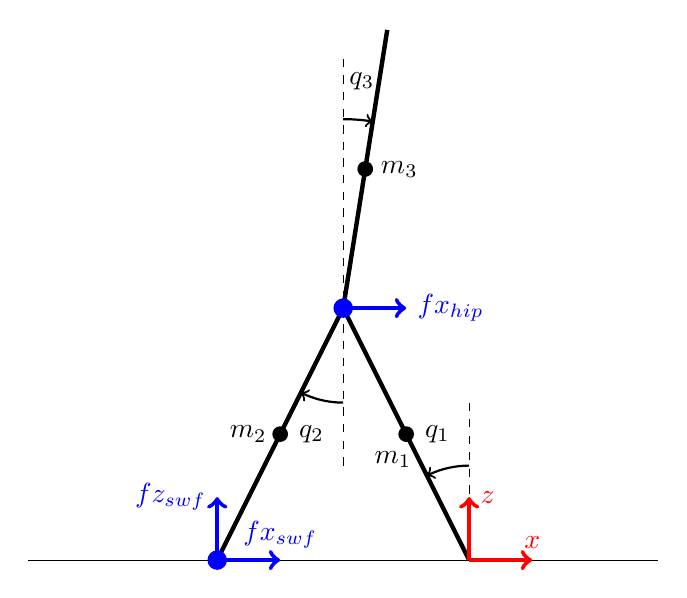
\begin{tikzpicture}
			\begin{scope}[x={8cm},y={8cm}]
				% l = 0,447213
				% alpha = 8.999999999478607 deg
				% =0.5+sqrt(0.2^2+0.4^2)*sin(pi/20)
				% =0.4+sqrt(0.2^2+0.4^2)*cos(pi/20)
				
				\draw[-] (0,0)--(1,0); % ground
				
				\draw[-,ultra thick] (0.3,0)--(0.5,0.4); % link 2
				\draw[-,ultra thick] (0.7,0)--(0.5,0.4); % link 1
				\draw[-,ultra thick] (0.5,0.4)--(0.5699596195707541,0.8417076540309386); % link 3
				
				\draw[dashed] (0.5,0.15)--(0.5,0.8); % big vertical dashed line
				\draw[dashed] (0.7,0)--(0.7,0.25); % small vertical dashed line
				
				\draw[->,ultra thick, red] (0.7,0)--(0.8,0) node[above]{$x$}; % x axis
				\draw[->,ultra thick, red] (0.7,0)--(0.7,0.1) node[right]{$z$}; % y axis
				
				\draw [->,thick,domain=-90:-116.5650512] plot ({0.5+0.15*cos(\x)}, {0.4+0.15*sin(\x)}); % q2
				\draw [->,thick,domain=90:116.5650512] plot ({0.7+0.15*cos(\x)}, {0.15*sin(\x)}); % q1
				\draw [->,thick,domain=90:81.00000000052139] plot ({0.5+0.3*cos(\x)}, {0.4+0.3*sin(\x)}); % q3
				
				\node at (0.4,0.2) [circle,fill,inner sep=1]{.}; % m2
				\node at (0.6,0.2) [circle,fill,inner sep=1]{.}; % m1
				\node at (0.5349798097853771,0.6208538270154693) [circle,fill,inner sep=1]{.}; % m3
				
				\node[text width=0mm] at (0.63,0.2) {$q_1$};
				\node[text width=0mm] at (0.43,0.2) {$q_2$};
				\node[text width=0mm] at (0.51,0.76) {$q_3$};
				
				\node[text width=0mm] at (0.55,0.16) {$m_1$};
				\node[text width=0mm] at (0.32,0.2) {$m_2$};
				\node[text width=0mm] at (0.56,0.62) {$m_3$};
				
				\node at (0.3,0) [circle,fill,inner sep=1.5, blue]{.};
				\node at (0.5,0.4) [circle,fill,inner sep=1.5, blue]{.};
				
				\draw[->,ultra thick, blue] (0.5,0.4)--(0.6,0.4) node[right]{$f{x_\text{hip}}$};
				\draw[->,ultra thick, blue] (0.3,0)--(0.4,0) node[above]{$f{x_\text{swf}}$};
				\draw[->,ultra thick, blue] (0.3,0)--(0.3,0.1) node[left]{$f{z_\text{swf}}$};
			\end{scope}
		\end{tikzpicture}
	\end{center}
	\caption{Representation of the three-link 2D biped model with the tasks forces used for the virtual model controller.}
	\label{fig::model_with_tasks}
\end{figure}


\paragraph{Command vector}

Finally, the command vector is computed as:

\begin{align*}
	\mathbf{u} &= \mathbf{u}_\text{top} + \mathbf{u}_\text{hip} + \mathbf{u}_\text{swf} \\
	&= \mathbf{u}_\text{top} + \mathbf{B}^+ \mathbf{J}_\text{hip}^T \mathbf{f}_\text{hip} + \mathbf{B}^+ \mathbf{J}_\text{swf}^T \mathbf{f}_\text{swf}
\end{align*}

and afterwards saturated to \SI{30}{\newton\meter}.

\paragraph{Optimization}
The optimization problem is defined as the objective function $f$ of the decision variables $p$ chosen amongst the model parameters:

\begin{align}
	\label{eq::virtual_model_objective_fun}
	f(p) &= w_1 d(p) + w_2 | \dot{x}_\text{hip d} - \bar{\dot{x}}_\text{hip}(p) | + w_3 \text{CMT}(p)^2 + w_4 | z_\text{hip d} - \bar{z}_\text{hip}(p) | + w_5 | z_\text{top d} - \bar{z}_\text{top}(p) | + w_6 | \text{step length}_\text{d} - \text{step length}|
\end{align}

where:

\begin{itemize}
	\item $d(p)$ the simulated total distance travelled by the robot,
	\item $\dot{x}_\text{hip d}$ is the desired horizontal hip velocity,
	\item $\bar{\dot{x}}_\text{hip} (p)$ the simulated average horizontal hip velocity,
	\item $z_\text{hip d}$ the desired vertical hip position,
	\item $\bar{z}_\text{hip}$ the simulated average vertical hip position,
	\item $z_\text{top d}$ the desired vertical top position,
	\item $\bar{z}_\text{top}$ the simulated average vertical top position,
	\item CMT$(p)$ the cost of mechanical transport as already defined,
	\item $\text{step length}_\text{d}$ the desired step length,
	\item step length the simulated average step length,
	\item and $w_i$ the weights.
\end{itemize}

\vspace{\baselineskip}

Many versions of this objective function were run, with various weights for each term, from 0 to cancel them out, to a much important proportion within $\sum w_i$.
In total, about thirty versions were optimized on five computers for a total of approximately fifty hours.

\paragraph{External forces}

After the final iteration of our optimizations was completed, the robustness of the controller to external forces was tested.
In order to do so, an external force of either \SI{100}{\newton} pushing, or \SI{-15}{\newton} pulling was applied to the hip at the beginning of a steady-state step for \SI{0.2}{\second}.

\paragraph{Internal forces}

And then, the robustness to measuring noise was tested as well, with centered gaussian noises applied to each $q_i$ and $\dot{q}_i$:

\begin{itemize}
	\item null average for both,
	\item 0.01 of variance for $q_i$,
	\item and 0.1 or variance for $\dot{q}_i$. 
\end{itemize}

The noise is continuously applied after reaching the steady-state.

\vspace{\baselineskip}

The values for both external and internal forces were chosen after several iterations to be close to the limits of the controller.